\documentclass[xcolor=dvipsnames]{beamer}

\usepackage{mpctools}
\usepackage{hyperref}

\setbeamertemplate{navigation symbols}{}
\newcommand{\clickurl}[1]{\href{#1}{\textcolor{blue}{\smallurl{#1}}}}

\begin{document}
%
\begin{frame}[allowframebreaks]{Installation}
    Install a scientific Python 2.7 distribution
    \begin{itemize}
        \item Any ``Scientific Python'' should do, but it must include NumPy, SciPy, matplotlib, and Tkinter.
        \item Be sure to choose 2.7 and not 3.x
        \item Spyder (a Python IDE) is very helpful but not required.
        \item See the \hyperlink{scientificpython}{\textcolor{blue}{Scientific Python Options}} slides for some good choices
    \end{itemize}
    
    \medskip
    
    Download our \texttt{mpctools} Python package
    \begin{itemize}
        \item Download zipped package: \clickurl{https://bitbucket.org/rawlings-group/mpc-tools-casadi}
        \begin{itemize}
            \item Click ``Downloads'' (cloud icon on left)
            \item Choose \texttt{mpc-tools-casadi.zip}
        \end{itemize}
        \item Unzip to a convenient location.
    \end{itemize}
    
    \framebreak
    
    Download \casadi{} (Version $\ge$3.0)
    \begin{itemize}
        \item Windows/Linux/Mac zip file available at \clickurl{http://files.casadi.org}
            \begin{itemize}
                \item Choose 3.1.1, pick OS, and download \texttt{casadi-py27-*.zip}
            \end{itemize}
        \item Unzip \texttt{casadi}, to the \texttt{mpc-tools-casadi} folder from the previous step.
    \end{itemize}
    
    \medskip
    
    Optional: Add CasADi and \texttt{mpctools} to your Python path
    \begin{itemize}
        \item Open a Python interpreter (run \lstinline[style=shell]!python! from a terminal/command prompt)
        \item Run the commands \lstinline[style=python]!import site; print site.getusersitepackages()! to see where your user site packages are stored
        \item Move the \texttt{casadi} and \texttt{mpctools} folders to that location.
        \begin{itemize}
            \item You should make the folders if they do not already exist
        \end{itemize}
    \end{itemize}
\end{frame}

\begin{frame}[allowframebreaks]{Scientific Python Options}
    \label{scientificpython}
    Anaconda (Linux, Windows, Mac)
    \begin{itemize}
        \item Download from \clickurl{https://www.continuum.io/downloads}
        \item Perhaps a bit bloated (contains packages we do not need)
        \item Typically the easiest version to work with.
    \end{itemize}
    
    \medskip
    
    APT (Ubuntu/Debian)
    \begin{itemize}
        \item Use \lstinline[style=shell]@sudo apt-get install spyder@ to get Spyder and all dependencies.
        \item Includes \texttt{python-numpy}, \texttt{python-scipy}, \texttt{python-matplotlib}, and \texttt{python-tk}.
    \end{itemize}
    
    \framebreak
    
    Miniconda (Linux, Windows, Mac)
    \begin{itemize}
        \item Smaller version of Anaconda
        \item Download from \clickurl{http://conda.pydata.org/miniconda.html}
        \item After install, need to install additional components
        \begin{itemize}
            \item Packages: \lstinline[style=shell]@conda install numpy scipy matplotlib tk@
            \item IDE: \lstinline[style=shell]@conda install spyder@
            \item Both commands should be entered in a terminal/command prompt
        \end{itemize}
    \end{itemize}
\end{frame}

\begin{frame}{Making Sure Everything Works}
    First, open a Python interpreter\footnote{Open a command prompt/terminal in the \smallurl{mpc-tools-casadi} folder and enter \lstinline[style=shell]!python!} and run \lstinline[style=python]!import casadi, mpctools!.
    \begin{itemize}
        \item If this doesn't work, make sure your CasADi folder shows up in \lstinline[style=python]!import sys; print sys.path!.
        \item If you have multiple Python distributions on your machine, don't (or at least make sure you're using the one you think you are).
        \item Make sure you are using Python 2.7 (not 3.x).
    \end{itemize}
    
    \medskip
    
    Then, try to run the examples in \smallurl{mpc-tools-casadi}.
    \begin{itemize}
        \item In the Python interpreter, use \lstinline[style=python]!execfile("filename.py")!.
        \item \smallurl{runall.py} will run everything and tell you if there are errors, but you won't see any plots.
    \end{itemize}
\end{frame}

\begin{frame}{Path Considerations}
    Unless you perform the optional step, \texttt{casadi} and \texttt{mpctools} are only accessible locally.
    \begin{itemize}
        \item Avoids cluttering Python system paths
        \item Doesn't need admin access
        \item To update, simply delete folders and re-download
        \item Python interpreter (or IDE) must be started from this folder
    \end{itemize}
    
    \medskip
    
    If you preform the optional step, \texttt{casadi} and \texttt{mpctools} will be accessible everywhere on your machine.
    \begin{itemize}
        \item Any Python interpreter can load the packages
        \item May be difficult to keep track of versions
        \item A local install will override a global install in the local directory
    \end{itemize}
\end{frame}

% Need this macro to split link across two lines.
\newcommand{\winsixtyfour}[1]{\href{https://sourceforge.net/projects/casadi/files/CasADi/commits/de2f632/windows/}{\textcolor{blue}{\footnotesize \texttt{#1}}}}
\begin{frame}[label=specialnotes]{Special Notes}
    The CasADi version you download must match the bitness of your Python installation (i.e., 32 vs. 64 bit).
    \begin{itemize}
        \item For 32 bit: \texttt{casadi-py27-np1.9.1-v3.1.1.zip}
        \item For 64 bit: \texttt{casadi-py27-np1.9.1-v3.1.1-64bit.zip}
        \item You can check Python bitness in an interpreter with \lstinline[style=python]!import sys; print 64 if sys.maxsize > 2**32 else 32!
    \end{itemize}
\end{frame}

\begin{frame}{Software Relationships}
    \centering
    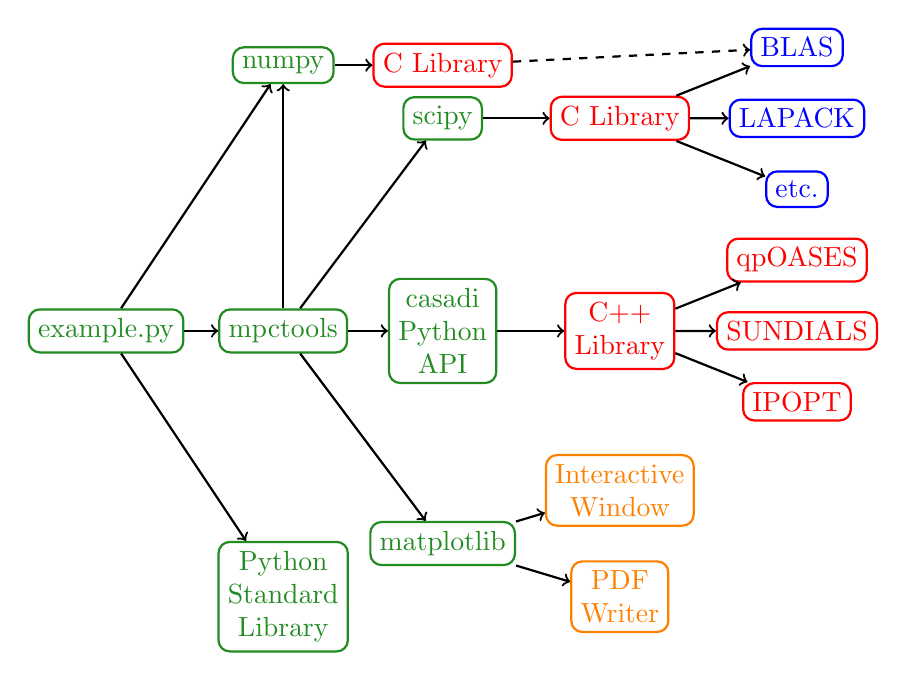
\begin{tikzpicture}
        [
            grow=right,
            code/.style={rectangle,rounded corners,align=center,thick},
            python/.style={code,draw=ForestGreen,text=ForestGreen},
            clib/.style={code,draw=Red,text=Red},
            fortran/.style={code,draw=Blue,text=Blue},
            backend/.style={code,draw=orange,text=orange},
            level 1/.style={level distance=2.5cm,sibling distance=3.75cm},
            level 2/.style={level distance=2.25cm,sibling distance=3cm},
            level 3/.style={level distance=2.5cm,sibling distance=1.5cm},
            level 4/.style={level distance=2.5cm,sibling distance=1cm},
            level 5/.style={level distance=2.5cm,sibling distance=1cm},
            arw/.style={->,thick},
            scale=.9,
        ]
        \draw (0,0) node[python] {example.py}
        child
        {
            node[python] {Python\\Standard\\Library}
            edge from parent [arw]
        }
        child
        {
            node[python] (mpc) {mpctools}
            child
            {
                node[python] (matplotlib) {matplotlib}
                child
                {
                    node [backend] {PDF\\Writer}
                    edge from parent [arw]
                }
                child
                {
                    node [backend] {Interactive\\Window}
                    edge from parent [arw]
                }
                edge from parent [arw]
            }
            child
            {
                node[python] (casadipy) {casadi\\Python\\API}
                child
                {
                    node[clib] {C++\\Library}
                    child
                    {
                        node[clib] {IPOPT}
                        edge from parent [arw]
                    }
                    child
                    {
                        node[clib] {SUNDIALS}
                        edge from parent [arw]
                    }
                    child
                    {
                        node[clib] {qpOASES}
                        edge from parent [arw]
                    }
                    edge from parent [arw]
                }
                edge from parent [arw]
            }
            child
            {
                node[python] (scipy) {scipy}
                child
                {
                    node[clib] {C Library}
                    child
                    {
                        node[fortran] {etc.}
                        edge from parent [arw]
                    }
                    child
                    {
                        node[fortran] {LAPACK}
                        edge from parent [arw]
                    }
                    child
                    {
                        node[fortran] (blas) {BLAS}
                        edge from parent [arw]
                    }
                    edge from parent [arw]
                }
                edge from parent [arw]
            }
            edge from parent [arw]
        }
        child
        {
            node[python] (numpy) {numpy}
            child
            {
                node[clib] (numpylib) {C Library}
                edge from parent [arw]
            }
            edge from parent [arw]
        };
        \draw[arw] (mpc) -- (numpy);
        \draw[arw,dashed] (numpylib) -- (blas);
    \end{tikzpicture}
\end{frame}
%
%
\end{document}